% Created by tikzDevice version 0.12.6 on 2026-08-03 04:28:46
% !TEX encoding = UTF-8 Unicode
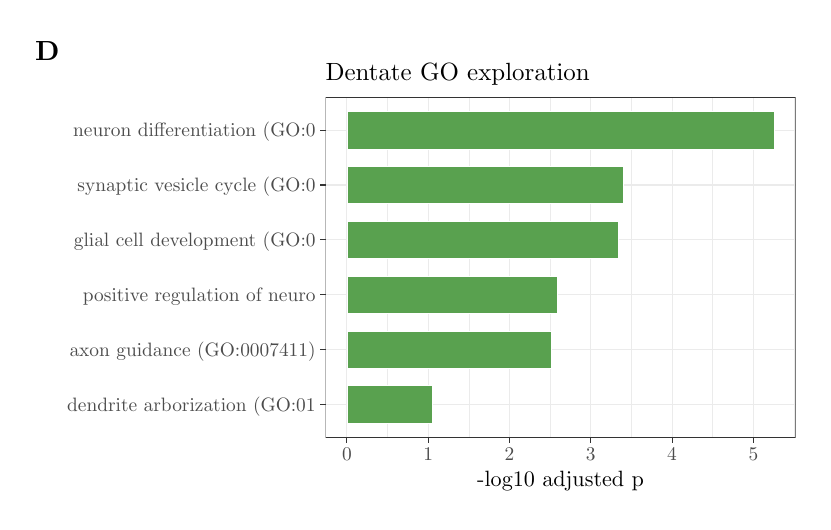
\begin{tikzpicture}[x=1pt,y=1pt]
\definecolor{fillColor}{RGB}{255,255,255}
\path[use as bounding box,fill=fillColor,fill opacity=0.00] (0,0) rectangle (280.14,171.36);
\begin{scope}
\path[clip] (  0.66,  1.87) rectangle (279.48,169.49);
\definecolor{drawColor}{RGB}{255,255,255}
\definecolor{fillColor}{RGB}{255,255,255}

\path[draw=drawColor,line width= 0.4pt,line join=round,line cap=round,fill=fillColor] (  0.66,  1.87) rectangle (279.48,169.49);
\end{scope}
\begin{scope}
\path[clip] (107.64, 23.34) rectangle (277.48,146.20);
\definecolor{fillColor}{RGB}{255,255,255}

\path[fill=fillColor] (107.64, 23.34) rectangle (277.48,146.20);
\definecolor{drawColor}{gray}{0.92}

\path[draw=drawColor,line width= 0.2pt,line join=round] (130.05, 23.34) --
	(130.05,146.20);

\path[draw=drawColor,line width= 0.2pt,line join=round] (159.42, 23.34) --
	(159.42,146.20);

\path[draw=drawColor,line width= 0.2pt,line join=round] (188.80, 23.34) --
	(188.80,146.20);

\path[draw=drawColor,line width= 0.2pt,line join=round] (218.17, 23.34) --
	(218.17,146.20);

\path[draw=drawColor,line width= 0.2pt,line join=round] (247.55, 23.34) --
	(247.55,146.20);

\path[draw=drawColor,line width= 0.2pt,line join=round] (276.92, 23.34) --
	(276.92,146.20);

\path[draw=drawColor,line width= 0.4pt,line join=round] (107.64, 35.23) --
	(277.48, 35.23);

\path[draw=drawColor,line width= 0.4pt,line join=round] (107.64, 55.04) --
	(277.48, 55.04);

\path[draw=drawColor,line width= 0.4pt,line join=round] (107.64, 74.86) --
	(277.48, 74.86);

\path[draw=drawColor,line width= 0.4pt,line join=round] (107.64, 94.67) --
	(277.48, 94.67);

\path[draw=drawColor,line width= 0.4pt,line join=round] (107.64,114.49) --
	(277.48,114.49);

\path[draw=drawColor,line width= 0.4pt,line join=round] (107.64,134.31) --
	(277.48,134.31);

\path[draw=drawColor,line width= 0.4pt,line join=round] (115.36, 23.34) --
	(115.36,146.20);

\path[draw=drawColor,line width= 0.4pt,line join=round] (144.74, 23.34) --
	(144.74,146.20);

\path[draw=drawColor,line width= 0.4pt,line join=round] (174.11, 23.34) --
	(174.11,146.20);

\path[draw=drawColor,line width= 0.4pt,line join=round] (203.49, 23.34) --
	(203.49,146.20);

\path[draw=drawColor,line width= 0.4pt,line join=round] (232.86, 23.34) --
	(232.86,146.20);

\path[draw=drawColor,line width= 0.4pt,line join=round] (262.23, 23.34) --
	(262.23,146.20);
\definecolor{drawColor}{RGB}{255,255,255}
\definecolor{fillColor}{RGB}{89,161,79}

\path[draw=drawColor,line width= 0.2pt,fill=fillColor] (115.36,127.57) rectangle (269.76,141.04);

\path[draw=drawColor,line width= 0.2pt,fill=fillColor] (115.36, 28.49) rectangle (146.25, 41.96);

\path[draw=drawColor,line width= 0.2pt,fill=fillColor] (115.36, 48.31) rectangle (189.03, 61.78);

\path[draw=drawColor,line width= 0.2pt,fill=fillColor] (115.36, 87.94) rectangle (213.47,101.41);

\path[draw=drawColor,line width= 0.2pt,fill=fillColor] (115.36, 68.12) rectangle (191.38, 81.60);

\path[draw=drawColor,line width= 0.2pt,fill=fillColor] (115.36,107.75) rectangle (215.14,121.23);
\definecolor{drawColor}{gray}{0.20}

\path[draw=drawColor,line width= 0.4pt,line join=round,line cap=round] (107.64, 23.34) rectangle (277.48,146.20);
\end{scope}
\begin{scope}
\path[clip] (  0.00,  0.00) rectangle (280.14,171.36);
\definecolor{drawColor}{gray}{0.30}

\node[text=drawColor,anchor=base east,inner sep=0pt, outer sep=0pt, scale=  0.70] at (104.04, 32.82) {dendrite arborization (GO:01};

\node[text=drawColor,anchor=base east,inner sep=0pt, outer sep=0pt, scale=  0.70] at (104.04, 52.63) {axon guidance (GO:0007411)};

\node[text=drawColor,anchor=base east,inner sep=0pt, outer sep=0pt, scale=  0.70] at (104.04, 72.45) {positive regulation of neuro};

\node[text=drawColor,anchor=base east,inner sep=0pt, outer sep=0pt, scale=  0.70] at (104.04, 92.26) {glial cell development (GO:0};

\node[text=drawColor,anchor=base east,inner sep=0pt, outer sep=0pt, scale=  0.70] at (104.04,112.08) {synaptic vesicle cycle (GO:0};

\node[text=drawColor,anchor=base east,inner sep=0pt, outer sep=0pt, scale=  0.70] at (104.04,131.90) {neuron differentiation (GO:0};
\end{scope}
\begin{scope}
\path[clip] (  0.00,  0.00) rectangle (280.14,171.36);
\definecolor{drawColor}{gray}{0.20}

\path[draw=drawColor,line width= 0.4pt,line join=round] (105.64, 35.23) --
	(107.64, 35.23);

\path[draw=drawColor,line width= 0.4pt,line join=round] (105.64, 55.04) --
	(107.64, 55.04);

\path[draw=drawColor,line width= 0.4pt,line join=round] (105.64, 74.86) --
	(107.64, 74.86);

\path[draw=drawColor,line width= 0.4pt,line join=round] (105.64, 94.67) --
	(107.64, 94.67);

\path[draw=drawColor,line width= 0.4pt,line join=round] (105.64,114.49) --
	(107.64,114.49);

\path[draw=drawColor,line width= 0.4pt,line join=round] (105.64,134.31) --
	(107.64,134.31);
\end{scope}
\begin{scope}
\path[clip] (  0.00,  0.00) rectangle (280.14,171.36);
\definecolor{drawColor}{gray}{0.20}

\path[draw=drawColor,line width= 0.4pt,line join=round] (115.36, 21.34) --
	(115.36, 23.34);

\path[draw=drawColor,line width= 0.4pt,line join=round] (144.74, 21.34) --
	(144.74, 23.34);

\path[draw=drawColor,line width= 0.4pt,line join=round] (174.11, 21.34) --
	(174.11, 23.34);

\path[draw=drawColor,line width= 0.4pt,line join=round] (203.49, 21.34) --
	(203.49, 23.34);

\path[draw=drawColor,line width= 0.4pt,line join=round] (232.86, 21.34) --
	(232.86, 23.34);

\path[draw=drawColor,line width= 0.4pt,line join=round] (262.23, 21.34) --
	(262.23, 23.34);
\end{scope}
\begin{scope}
\path[clip] (  0.00,  0.00) rectangle (280.14,171.36);
\definecolor{drawColor}{gray}{0.30}

\node[text=drawColor,anchor=base,inner sep=0pt, outer sep=0pt, scale=  0.70] at (115.36, 14.92) {0};

\node[text=drawColor,anchor=base,inner sep=0pt, outer sep=0pt, scale=  0.70] at (144.74, 14.92) {1};

\node[text=drawColor,anchor=base,inner sep=0pt, outer sep=0pt, scale=  0.70] at (174.11, 14.92) {2};

\node[text=drawColor,anchor=base,inner sep=0pt, outer sep=0pt, scale=  0.70] at (203.49, 14.92) {3};

\node[text=drawColor,anchor=base,inner sep=0pt, outer sep=0pt, scale=  0.70] at (232.86, 14.92) {4};

\node[text=drawColor,anchor=base,inner sep=0pt, outer sep=0pt, scale=  0.70] at (262.23, 14.92) {5};
\end{scope}
\begin{scope}
\path[clip] (  0.00,  0.00) rectangle (280.14,171.36);
\definecolor{drawColor}{RGB}{0,0,0}

\node[text=drawColor,anchor=base,inner sep=0pt, outer sep=0pt, scale=  0.80] at (192.56,  5.64) {-log10 adjusted p};
\end{scope}
\begin{scope}
\path[clip] (  0.00,  0.00) rectangle (280.14,171.36);
\definecolor{drawColor}{RGB}{0,0,0}

\node[text=drawColor,anchor=base west,inner sep=0pt, outer sep=0pt, scale=  0.90] at (107.64,152.18) {Dentate GO exploration};
\end{scope}
\begin{scope}
\path[clip] (  0.00,  0.00) rectangle (280.14,171.36);
\definecolor{drawColor}{RGB}{0,0,0}

\node[text=drawColor,anchor=base,inner sep=0pt, outer sep=0pt, scale=  1.00] at (  7.07,159.49) {\bfseries D};
\end{scope}
\end{tikzpicture}
